
%%%%%%%%%%%%%%%%%%%%%%%%%%%%%%%%%%%%%%%%%%%%%%%%%%%%%%%%%%%%%%%%%%%%%
% FOR PRINTING
\documentclass[
    11pt,
    a4paper,
    openright,
    cleardoubleplain,
    appendixprefix,
    chapterprefix,
    numbers=noenddot,
    DIV11,
    BCOR15mm
]{report}
               
\newcommand{\litl}{LiTL}
\newcommand{\reporttitle}{\litl}               
\newcommand{\reportsubtitle}{Lightweight Trace Library}
\newcommand{\reportsubsubtitle}{User Manual}
%%%%%%%%%%%%%%%%%%%%%%%%%%%%%%%%%%%%%%%%%%%%%%%%%%%%%%%%%%%%%%%%%%%%%
\usepackage{etex}
\usepackage{savesym}
\usepackage[utf8]{inputenc}

\usepackage[T1]{fontenc}
\usepackage[small,bf]{caption}

% for plotting 
\usepackage{tikz}
\usepackage{pgfplots}
\usepackage{subfigure}
\usepackage{graphicx}
\usepackage{color}
\usepackage{xcolor}
    \definecolor{ListingsKeywordColor}{rgb}{0,0,0.4}
    \definecolor{ListingsIdentifierColor}{rgb}{0,0.5,0}
    \definecolor{ListingsCommentColor}{rgb}{0.4,0.4,0.4}
    \definecolor{ListingsStringColor}{rgb}{0.6000,0.3333,0.7333}%{0.8,0,0}
    \definecolor{ListingsRuleSepColor}{rgb}{0,0,0}
    \definecolor{ListingsEmphColor}{rgb}{0,0.6667,0.6667}
    \definecolor{ListingsBreakSymbolColor}{rgb}{0.780,0.082,0.522}
    \definecolor{LinkColor}{rgb}{0,0,0.5}
    \definecolor{UnitColor}{rgb}{0,0,0}
    \definecolor{MathsVectorColor}{rgb}{0,0,0}
    \definecolor{MathsMatrixColor}{rgb}{0,0,0}
    \definecolor{MyGreen}{HTML}{228B22}
%     \definecolor{TikzGreen}{HTML}{}
    \definecolor{MyBlue}{HTML}{0000FF}
    \colorlet{MatrixElementsLight}{gray!20!white}
    \colorlet{MatrixElementsDark}{gray!40}

% for listing
\usepackage{listings}
  \lstset{
    basicstyle=\scriptsize\ttfamily,
    tabsize=3,
    showtabs=false,
    showspaces=false,
    showstringspaces=false,
    tab=\rightarrowfill,
    keywordstyle=\color{ListingsKeywordColor},
    identifierstyle=\color{ListingsIdentifierColor},
    commentstyle=\color{ListingsCommentColor},
    stringstyle=\color{ListingsStringColor},
    emphstyle=\color{ListingsEmphColor}\bfseries\underbar,
    frame=none,
    rulesepcolor=\color{ListingsRuleSepColor},
    numbers=left,
    numberstyle=\tiny,
    numbersep=5pt,
    captionpos=top,
    frame=tb,
    firstnumber=1,
    stepnumber=1,
%     numberfirstline=false,
    breaklines=true,
    breakatwhitespace=true,
%     prebreak=\mbox{\,$\color{ListingsBreakSymbolColor}\mathbf{\hookleftarrow}$},
    mathescape=true,
    morekeywords={},
}

\usepackage{url}
\usepackage[final]{hyperref}
\hypersetup{
   % Farben fuer die Links
   colorlinks=false,         % Links erhalten Farben statt Kaeten
   urlcolor=LinkColor,    % \href{...}{...} external (URL)
   filecolor=LinkColor,  % \href{...} local file
   linkcolor=LinkColor,  %\ref{...} and \pageref{...}
   menucolor=LinkColor,
   citecolor=LinkColor,
   % Links
   raiselinks=true,       % calculate real height of the link
   breaklinks,              % Links berstehen Zeilenumbruch
   %backref=page,            % Backlinks im Literaturverzeichnis (section, slide, page, none)
   %pagebackref=true,        % Backlinks im Literaturverzeichnis mit Seitenangabe
   verbose,
   hyperindex=true,         % backlinkex index
   linktocpage=true,        % Inhaltsverzeichnis verlinkt Seiten
   hyperfootnotes=false,     % Keine Links auf Fussnoten
   % Bookmarks
   bookmarks=true,          % Erzeugung von Bookmarks fuer PDF-Viewer
   bookmarksopenlevel=1,    % Gliederungstiefe der Bookmarks
   bookmarksopen=false,      % Expandierte Untermenues in Bookmarks
   bookmarksnumbered=true,  % Nummerierung der Bookmarks
   bookmarkstype=toc,       % Art der Verzeichnisses
   % Anchors
   plainpages=false,        % Anchors even on plain pages ?
   pageanchor=true,         % Pages are linkable
   % PDF Informationen
   pdftitle={\reporttitle: \reportsubtitle. \reportsubsubtitle},             % Titel
   pdfauthor={Roman Iakymchuk},            % Autor
   pdfcreator={LaTeX, hyperref, KOMA-Script},
   pdfstartview=Fit,       % Dokument wird Fit Height geaefnet
   pdffitwindow=true,
   pdfpagemode=UseOutlines, % Bookmarks im Viewer anzeigen
   pdfpagelabels=true,      % set PDF page labels
}

\usepackage{cleveref}
\Crefname{algorithm}{Alg.}{Algs.}
\Crefname{figure}{Fig.}{Figs.}
\Crefname{table}{Tab.}{Tabs.}
\Crefname{equation}{Eq.}{Eqs.}
\Crefname{eqnarray}{Eq.}{Eqs.}

\usepackage{float}
\newfloat{algorithm}{htb}{lob}
\floatname{algorithm}{Algorithm}

\newlength{\figlength}
\setlength{\figlength}{7.6cm} %8.2cm
\newlength{\subfiglength}
\setlength{\subfiglength}{7.3cm}%7.8

\newcommand{\bytes}{b}
\newcommand{\kb}{Kb}
\newcommand{\mb}{Mb}
\newcommand{\ghz}{GHz}
\newcommand{\flop}{Flop}
\newcommand{\flops}{Flops}
\newcommand{\gflops}{G\flops}
\newcommand{\eztrace}{EZTrace}
\newcommand{\fxt}{FxT}
\newcommand{\pthread}{Pthreads}
\newcommand{\openmp}{OpenMP}
\newcommand{\mpi}{MPI}
\newcommand{\dash}{ -- }


% Title Page
\title{
{\Huge\bf \reporttitle{}}\\[6mm]
{\LARGE\bf \reportsubtitle}\\[12mm]
{\Large\bf \reportsubsubtitle}}
\author{Roman Iakymchuk and Fran\c{c}ois Trahay}

\begin{document}
\hypersetup{pageanchor=false}
\maketitle
\hypersetup{pageanchor=true}

% \setcounter{page}{2}
\tableofcontents

\chapter{License of \litl}
\litl{} is developed and distributed under the GNU General Public License.

This library is free software; you can redistribute it and/or modify it under 
the terms of the GNU General Public License as published by the Free Software 
Foundation; either version 2 of the License, or (at your option) any later 
version.

\litl{} is distributed in the hope that it will be useful, but WITHOUT ANY 
WARRANTY; without even the implied warranty of MERCHANTABILITY or FITNESS FOR A 
PARTICULAR PURPOSE. See the GNU General Public License for more details.

You should have received a copy of the GNU General Public License along with 
\litl{}; if not, write to the Free Software Foundation, Inc., 675 Mass Ave, 
Cambridge, MA 02139, USA.


\chapter{Overview of \litl}
\litl{}~\cite{litl} is a lightweight binary trace library that aims at 
providing performance analysis tools with a scalable event recording mechanism 
that utilizes minimum resources of the CPU and memory. In order to efficiently 
analyze modern HPC applications that combine \openmp{} (or \pthread) threads 
and \mpi{} processes, we design and implement various mechanisms to ensure the 
scalability of \litl{} for a large  number of both threads and processes. 

\litl{} is designed in order to resolve the following performance tracing 
issues:
\begin{itemize}
 \item Scalability and the number of threads;
 \item Scalability and the number of recorded traces;
 \item Optimization in the storage capacity usage.
\end{itemize}
As a result, \litl{} provides similar functionality to standard event recording 
libraries and records events only from user-space. \litl{} minimizes the usage 
of the CPU time and memory space in order to avoid disturbing the application 
that is being analyzed. Also, \litl{} is fully thread-safe that allows to record 
events from multi-threaded applications. Finally, \litl{} is a generic library 
that can be used in conjunction with many performance analysis tools and 
frameworks. 


\chapter{Installation}
\section{Requirements}
In order to use \litl{}, the following software is required:
\begin{enumerate}
 \item autoconf of version 2.63;
 
\end{enumerate}

\section{Getting \litl}
Current development version of \litl{} is available via Git\\
    \hspace*{0.9cm}\texttt{git clone git+ssh://fusionforge.int-evry.fr//var/lib/}\\
    \hspace*{0.9cm}\texttt{gforge/chroot/scmrepos/git/litl/litl.git}\\
After getting the latest development version from Git, the following command 
should be run\\
\hspace*{0.9cm}\texttt{./bootstrap}\\ 
And, only afterwards the tool can be built.

\section{Building \eztrace{}}
At first, to configure \litl{} the following configure script should be 
invoked\\
    \hspace*{0.9cm}\texttt{./configure -\,-prefix=<LITL\_INSTALL\_DIR>}\\
The configuration script contains many different options that can be set. 
However, during the first try we recommend to use the default settings.

Once \litl{} is configured, the next two commands should be executed to complete  
the building\\
    \hspace*{0.9cm}\texttt{make}\\
    \hspace*{0.9cm}\texttt{make install}

In order to check whether \litl{} was installed correctly, a set of tests can be 
run as\\
    \hspace*{0.9cm}\texttt{make check}


\chapter{How to Use \litl{}?}
\section{Reading Events}
After the application was traced and events were recorded into binary trace 
files, those traces can be analyzed using \texttt{litl\_read} as\\
    \hspace*{0.9cm}\texttt{litl\_read -f trace.file}\\
This utility shows the recorded events in the following format:
\begin{itemize}
 \item Time since last probe record on the same CPU;
 \item ID of the current thread on this CPU;
 \item Event type;
 \item Code of the probe;
 \item Number of parameters of the probe;
 \item List of parameters of the probe, if any.
\end{itemize}

\section{Merging Traces}
Once the traces were recorded, they can be merged into an archive of traces for
further processing by the following command\\
    \hspace*{0.9cm}\texttt{litl\_read  -o archive.trace trace.0 trace.1 ... trace.n}

\section{Splitting Traces}
In case of a need for a detailed analysis of a particular trace files, an archive
of traces can be split back into separate traces by\\
\hspace*{0.9cm}\texttt{litl\_read  -f archive.trace -d output.dir}

\section{Environment Variables}
For a more flexible and comfortable usage of \litl{}, we provide the following 
environment variables:
\begin{itemize}
 \item \texttt{LITL\_BUFFER\_SIZE} provides users with the alternative 
       possibility to set a buffer size. If the variable is not specified, then 
       the provided value inside the application is used;
       
 \item \texttt{LITL\_BUFFER\_FLUSH} specifies the behavior of \litl{} when the 
       event buffer is full. If it is set to ``on'', which is a default option, 
       the buffer is flushed. This permits to record traces that are larger 
       than the buffer size. Otherwise, if it is set to ``off'', any additional 
       event will not be recorded. The trace is, thus, truncated and there is no 
       impact on the application performance;
      
 \item \texttt{LITL\_TID\_RECORDING} provides users with an alternative 
       possibility to enable or disable tid recording. If it is set to ``on'', 
       which is a default value, the tid recording is enabled. Otherwise, when 
       it is set to ``off'', the tid recording is disable;

 \item \texttt{LITL\_THREAD\_SAFETY} specifies the behavior of \litl{} while
       tracing multi-threaded applications. If it is set to ``on'', which is a 
       default value, the thread safety is enabled. Otherwise, when it is set to
       ``off'', the event recording is not thread safe;
 
 \item \texttt{LITL\_TIMING\_METHOD} specifies the timing method that will be 
       used during the recording phase. The \litl{} timing methods can be 
       divided into two groups: those that measure time in clock ticks and 
       those that rely on the \texttt{clock\_gettime()} function. The first 
       group has only one method:
       \begin{itemize}
        \item \texttt{ticks} that uses the CPU specific register, e.g. rdtsc 
        on X86 and X86\_64 architectures.
       \end{itemize}     
       The second group comprises of the other five different methods:
       \begin{itemize}
        \item \texttt{monotonic} that corresponds to \texttt{CLOCK\_MONOTONIC};
        \item \texttt{monotonic\_raw}\dash{}\texttt{CLOCK\_MONOTONIC\_RAW};
        \item \texttt{realtime}\dash{}\texttt{CLOCK\_REALTIME};
        \item \texttt{thread\_cputime}\dash{}\texttt{CLOCK\_THREAD\_CPUTIME\_ID};        
        \item \texttt{process\_cputime}\dash{}\texttt{CLOCK\_PROCESS\_CPUTIME\_ID}.
       \end{itemize}
       User can also define its own timing method and set the environment 
       variable accordingly.
\end{itemize}


\chapter{\litl{} in Details}
\section{Event Types and The Storage Usage}
Each event in the \litl{} library consists of two parts: the event core (the 
event code, the time when the event occurred, the thread identifier, and the 
number of parameters) and event parameters. The number of event parameters 
recorded by \litl{} varies from zero to ten. 

The parameters passed to each event have different data type. In order to handle
the variety of possible cases, event's parameters in \litl{} can be represented 
by the largest data type, which is \texttt{uint64\_t} on x86\_64 architectures.
Hence, any parameter -- no matter whether it is a \texttt{char}, an 
\texttt{int} or a \texttt{long int} -- can be recorded without being truncated. 
However, the reserved slot for each parameter is often bigger than its actual 
size. Thus, this leads to the non-optimal usage of resources.
Our goal is to keep trace files as small as possible without 
losing any of the recorded data. Therefore, we propose to use the compacted 
event storage that aims at utilizing every byte from the allocated space.

In our approach, we introduce three different types of events: regular, raw, and
packed. The regular event is without any major optimization being involved. 
The raw event stores parameters in the string format. Its purpose is to gather 
either the regular parameters in a string format or the information about the 
abnormal behavior of applications like thrown exceptions.
The packed event represents the optimized versions of storing events, where 
each parameter can be saved as a group of bytes. Accordingly, by using the 
event type packed for recording and storing events, we theoretically are 
capable to save up to 65\,\% of the disk space compare to the regular \litl{}.

\Cref{fig:event_storage_fxt} shows, on an example of three regular events with 
different number of parameters, the occupied space of events within the trace 
file recorded by \eztrace\ with \litl{}. We symbolically partitioned the trace 
file into bytes and also chunks of bytes, which store event's components. The 
space occupied by each event is highlighted with parentheses.

\begin{landscape}

\begin{figure}[!t]
\begin{center}
  \begin{footnotesize}
\subfigure[Regular Events]{
    \label{fig:event_storage_fxt}
    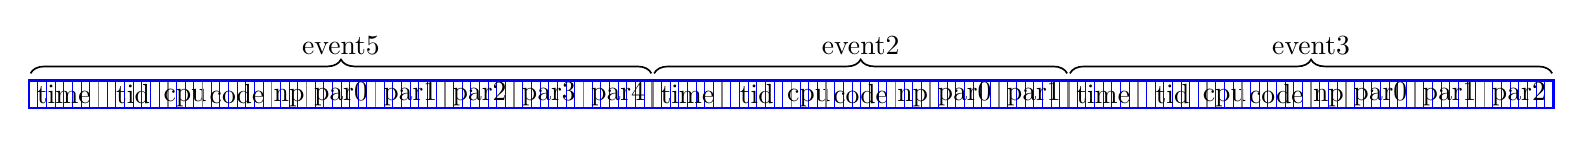
\begin{tikzpicture}[scale=.88]
    % vertical lines
    \foreach \x in {.125,.25,...,21.875}
        \draw[blue,line width=.12mm](\x,1.2) -- (\x,1.6);gray
    % event5
    \draw [
    semithick,
    decorate,
    decoration={
        brace,
        amplitude=5pt,
        raise=-0.35cm
    }] (0.02,2.1) -- (8.98, 2.1) node[midway]{event5}; 
    \draw (0.5, 1.4) -- (0.5, 1.4) node{time};
    \draw[gray,line width=.2mm](1.,1.2) -- (1.,1.6);
    \draw (1.5, 1.4) -- (1.5, 1.4) node{tid};
    \draw[gray,line width=.2mm](2.,1.2) -- (2.,1.6);
    \draw (2.25, 1.35) -- (2.25, 1.35) node{cpu};
    \draw[gray,line width=.2mm](2.5,1.2) -- (2.5,1.6);  
    \draw (3., 1.4) -- (3., 1.4) node{code};
    \draw[gray,line width=.2mm](3.5,1.2) -- (3.5,1.6);
    \draw (3.75, 1.35) -- (3.75, 1.35) node{np};
    \draw[gray,line width=.2mm](4.,1.2) -- (4.,1.6);    
    \draw (4.5, 1.4) -- (4.5, 1.4) node{par0};
    \draw[gray,line width=.2mm](5.,1.2) -- (5.,1.6);
    \draw (5.5, 1.4) -- (5.5, 1.4) node{par1};
    \draw[gray,line width=.2mm](6.,1.2) -- (6.,1.6);
    \draw (6.5, 1.4) -- (6.5, 1.4) node{par2};
    \draw[gray,line width=.2mm](7.,1.2) -- (7.,1.6);  
    \draw (7.5, 1.4) -- (7.5, 1.4) node{par3};
    \draw[gray,line width=.2mm](8.,1.2) -- (8.,1.6);
    \draw (8.5, 1.4) -- (8.5, 1.4) node{par4};
    \draw[gray,line width=.4mm](9.,1.2) -- (9.,1.6);    
    % event2
    \draw [
    semithick,
    decorate,
    decoration={
        brace,
        amplitude=5pt,
        raise=-0.35cm
    }] (9.02,2.1) -- (14.98, 2.1) node[midway]{event2};     
    \draw (9.5, 1.4) -- (9.5, 1.4) node{time};
    \draw[gray,line width=.2mm](10.,1.2) -- (10.,1.6);
    \draw (10.5, 1.4) -- (10.5, 1.4) node{tid};
    \draw[gray,line width=.2mm](11.,1.2) -- (11.,1.6);
    \draw (11.25, 1.35) -- (11.25, 1.35) node{cpu};
    \draw[gray,line width=.2mm](11.5,1.2) -- (11.5,1.6);  
    \draw (12., 1.4) -- (12., 1.4) node{code};
    \draw[gray,line width=.2mm](12.5,1.2) -- (12.5,1.6);
    \draw (12.75, 1.35) -- (12.75, 1.35) node{np};
    \draw[gray,line width=.2mm](13.,1.2) -- (13.,1.6);
    \draw (13.5, 1.4) -- (13.5, 1.4) node{par0};
    \draw[gray,line width=.2mm](14.,1.2) -- (14.,1.6);    
    \draw (14.5, 1.4) -- (14.5, 1.4) node{par1};
    \draw[gray,line width=.4mm](15.,1.2) -- (15.,1.6);    
    % event3
    \draw [
    semithick,
    decorate,
    decoration={
        brace,
        amplitude=5pt,
        raise=-0.35cm
    }] (15.02,2.1) -- (21.98, 2.1) node[midway]{event3};         
    \draw (15.5, 1.4) -- (15.5, 1.4) node{time};
    \draw[gray,line width=.2mm](16.,1.2) -- (16.,1.6);
    \draw (16.5, 1.4) -- (16.5, 1.4) node{tid};
    \draw[gray,line width=.2mm](17.,1.2) -- (17.,1.6);
    \draw (17.25, 1.35) -- (17.25, 1.35) node{cpu};
    \draw[gray,line width=.2mm](17.5,1.2) -- (17.5,1.6);  
    \draw (18., 1.4) -- (18., 1.4) node{code};
    \draw[gray,line width=.2mm](18.5,1.2) -- (18.5,1.6);
    \draw (18.75, 1.35) -- (18.75, 1.35) node{np};
    \draw[gray,line width=.2mm](19.,1.2) -- (19.,1.6);
    \draw (19.5, 1.4) -- (19.5, 1.4) node{par0};
    \draw[gray,line width=.2mm](20.,1.2) -- (20.,1.6);    
    \draw (20.5, 1.4) -- (20.5, 1.4) node{par1};
    \draw[gray,line width=.2mm](21.,1.2) -- (21.,1.6);    
    \draw (21.5, 1.4) -- (21.5, 1.4) node{par2};
    % big rectangle
    \draw [blue, line width=.3mm]
        (0.,1.2) rectangle (22.,1.6);
           
    \end{tikzpicture}
}
\subfigure[Packed Events]{
    \label{fig:event_storage_litl}
    \hspace*{2mm}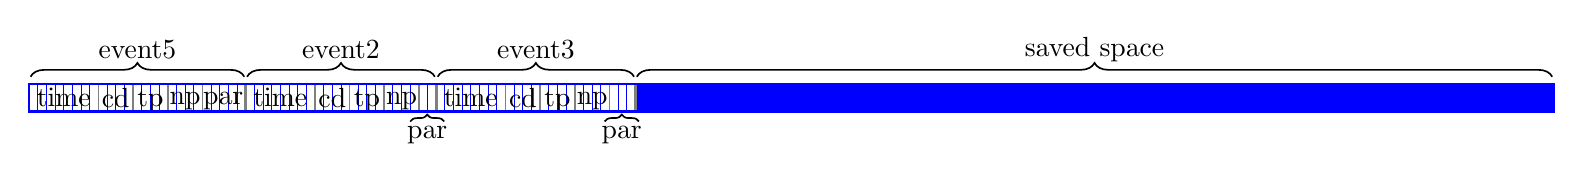
\begin{tikzpicture}[scale=.88]
    % vertical lines
    \foreach \x in {.125,.25,...,21.875}
        \draw[blue,line width=.12mm](\x,1.2) -- (\x,1.6);gray
    % event5
    \draw [
    semithick,
    decorate,
    decoration={
        brace,
        amplitude=5pt,
        raise=-0.35cm
    }] (0.02,2.1) -- (3.105, 2.1) node[midway]{event5}; 
    \draw (0.5, 1.4) -- (0.5, 1.4) node{time};
    \draw[gray,line width=.2mm](1.,1.2) -- (1.,1.6);
    \draw (1.25, 1.4) -- (1.25, 1.4) node{cd};
    \draw[gray,line width=.2mm](1.5,1.2) -- (1.5,1.6);
    \draw (1.75, 1.36) -- (1.75, 1.36) node{tp};
    \draw[gray,line width=.2mm](2.,1.2) -- (2.,1.6);  
    \draw (2.25, 1.35) -- (2.25, 1.35) node{np};
    \draw[gray,line width=.2mm](2.5,1.2) -- (2.5,1.6);
    \draw (2.8, 1.35) -- (2.8, 1.35) node{par};
    \draw[gray,line width=.4mm](3.125,1.2) -- (3.125,1.6);
    % event2
    \draw [
    semithick,
    decorate,
    decoration={
        brace,
        amplitude=5pt,
        raise=-0.35cm
    }] (3.145,2.1) -- (5.855, 2.1) node[midway]{event2};     
    \draw (3.625, 1.4) -- (3.625, 1.4) node{time};
    \draw[gray,line width=.2mm](4.125,1.2) -- (4.125,1.6);
    \draw (4.375, 1.4) -- (4.375, 1.4) node{cd};
    \draw[gray,line width=.2mm](4.625,1.2) -- (4.625,1.6);
    \draw (4.875, 1.36) -- (4.875, 1.36) node{tp};
    \draw[gray,line width=.2mm](5.125,1.2) -- (5.125,1.6);  
    \draw (5.375, 1.35) -- (5.375, 1.35) node{np};
    \draw[gray,line width=.2mm](5.625,1.2) -- (5.625,1.6);
    \draw [
    semithick,
    decorate,
    decoration={
        brace,
        amplitude=2.5pt,
        raise=-0.065cm
    }] (5.5,1.13) -- (5.99, 1.13) node[midway,below]{par}; 
    \draw[gray,line width=.4mm](5.875,1.2) -- (5.875,1.6);
    % event3
    \draw [
    semithick,
    decorate,
    decoration={
        brace,
        amplitude=5pt,
        raise=-0.35cm
    }] (5.895,2.1) -- (8.73, 2.1) node[midway]{event3};         
    \draw (6.375, 1.4) -- (6.375, 1.4) node{time};
    \draw[gray,line width=.2mm](6.875,1.2) -- (6.875,1.6);
    \draw (7.125, 1.4) -- (7.125, 1.4) node{cd};
    \draw[gray,line width=.2mm](7.375,1.2) -- (7.375,1.6);
    \draw (7.625, 1.36) -- (7.625, 1.36) node{tp};
    \draw[gray,line width=.2mm](7.875,1.2) -- (7.875,1.6);  
    \draw (8.125, 1.35) -- (8.125, 1.35) node{np};
    \draw[gray,line width=.2mm](8.375,1.2) -- (8.375,1.6);
    \draw [
    semithick,
    decorate,
    decoration={
        brace,
        amplitude=2.5pt,
        raise=-0.065cm
    }] (8.305,1.13) -- (8.8, 1.13) node[midway,below]{par};     
    \draw[gray,line width=.4mm](8.75,1.2) -- (8.75,1.6);
    % saved space
    \draw [
    semithick,
    decorate,
    decoration={
        brace,
        amplitude=5pt,
        raise=-0.35cm
    }] (8.77,2.1) -- (21.98, 2.1) node[midway]{saved space};
    % gray rectangle
    \draw [gray, fill=blue, line width=.12mm]
        (8.77,1.2) rectangle (22.,1.6);     
    % big rectangle
    \draw [blue, line width=.3mm]
        (0.,1.2) rectangle (22.,1.6);
           
    \end{tikzpicture}
}
  \end{footnotesize}  
\caption{Storage of different kinds of events in the trace file. 
In the figure, \emph{time} is the time when the event occurred; 
\emph{cd} means the event code; \emph{tp} is the event type; \emph{np} stands 
for the number of event's parameters; \emph{par}\dash{}an array of parameters.}
\label{fig:event_storage_all}
\end{center}
\end{figure}


\begin{figure*}[!t]
\begin{center}
  \begin{footnotesize}
    \hspace*{-1mm}
    \begin{tikzpicture}[scale=1.2]
    \draw [blue, fill=MatrixElementsDark, line width=.35mm, rounded corners]
        (0.,0.) rectangle (18.5,1.);
    % header
    \draw [MyGreen, fill=white, line width=.3mm, rounded corners]
        (0.1,0.1) rectangle (8.4,.9);
    \draw [MyGreen, line width=.3mm] (.1, .6) -- (8.4, .6);
    \draw (4.2, .73) -- (4.2, .73) node{H    E    A    D    E    R};
    % litl version and OS
    \draw [gray, fill=white, line width=.3mm, rounded corners]
        (.15,0.15) rectangle (1.15,.55);
    %\draw (.65, .35) -- (.65, .35) node{\litl{\_}v};    
    \node at (.65, .35) {\litl{\_}v};
    \draw [gray, fill=white, line width=.3mm, rounded corners]
        (1.2,0.15) rectangle (1.6,.55);
    \draw (1.4, .35) -- (1.4, .35) node{OS};        
    % buffer size and #threads
    \draw [gray, fill=white, line width=.3mm, rounded corners]
        (1.65,0.15) rectangle (2.75,.55);
    \draw (2.2, .35) -- (2.2, .35) node{\#threads};    
    \draw [gray, fill=white, line width=.3mm, rounded corners]
        (2.8,0.15) rectangle (3.85,.55);
    \draw (3.33, .35) -- (3.33, .35) node{buf\_size};
    % tids and offsets
    \draw [gray, fill=white, line width=.3mm, rounded corners]
        (3.9,0.15) rectangle (5.35,.55);
    \draw (4.2, .35) -- (4.2, .35) node{tid0};
    \draw [gray, line width=.3mm] (4.46, .15) -- (4.46, .55);
    \node at (4.93, .35) {offset0};
    
    \draw [gray, fill=white, line width=.3mm, rounded corners]
        (5.4,0.15) rectangle (6.85,.55);
    \draw (5.7, .35) -- (5.7, .35) node{tid1};
    \draw [gray, line width=.3mm] (5.96, .15) -- (5.96, .55);
    \draw (6.43, .35) -- (6.43, .35) node{offset1};
    
    \draw [gray, fill=white, line width=.3mm, rounded corners]
        (6.9,0.15) rectangle (8.35,.55);
    \draw (7.2, .35) -- (7.2, .35) node{tid2};
    \draw [gray, line width=.3mm] (7.46, .15) -- (7.46, .55);
    \draw (7.93, .35) -- (7.93, .35) node{offset2};
    % chunk00
    \draw [MyGreen, fill=white, line width=.3mm, rounded corners]
        (8.5,0.1) rectangle (10.4,.9);
    \draw [MyGreen, line width=.3mm] (8.5, .6) -- (10.4, .6);
    \node at (8.65,0.9) (chunk00) {};
    \draw (9.45, .73) -- (9.45, .73) node{chunk00};
    \draw [gray, fill=white, line width=.3mm, rounded corners]
        (8.55,0.15) rectangle (9.35,.55);
    \draw (8.95, .35) -- (8.95, .35) node{events};
    \draw [gray, fill=white, line width=.3mm, rounded corners]
        (9.4,0.15) rectangle (10.35,.55);
    \draw (9.88, .35) -- (9.88, .35) node{offset01};
    % chunk20
    \draw [MyGreen, fill=white, line width=.3mm, rounded corners]
        (10.5,0.1) rectangle (12.4,.9);
    \draw [MyGreen, line width=.3mm] (10.5, .6) -- (12.4, .6);
    \draw (11.45, .73) -- (11.45, .73) node{chunk20};
    \node at (10.65,0.9) (chunk20) {};
    \draw [gray, fill=white, line width=.3mm, rounded corners]
        (10.55,0.15) rectangle (11.35,.55);
    \draw (10.95, .35) -- (10.95, .35) node{events};
    \draw [gray, fill=white, line width=.3mm, rounded corners]
        (11.4,0.15) rectangle (12.35,.55);
    \draw (11.88, .35) -- (11.88, .35) node{offset21};
    % chunk01
    \draw [MyGreen, fill=white, line width=.3mm, rounded corners]
        (12.5,0.1) rectangle (14.4,.9);
    \draw [MyGreen, line width=.3mm] (12.5, .6) -- (14.4, .6);
    \draw (13.45, .73) -- (13.45, .73) node{chunk01};
    \node at (12.65,0.9) (chunk01) {};
    \draw [gray, fill=white, line width=.3mm, rounded corners]
        (12.55,0.15) rectangle (13.35,.55);
    \draw (12.95, .35) -- (12.95, .35) node{events};
    \draw [gray, fill=white, line width=.3mm, rounded corners]
        (13.4,0.15) rectangle (14.35,.55);
    \draw (13.88, .35) -- (13.88, .35) node{offset02};
    % chunk10
    \draw [MyGreen, fill=white, line width=.3mm, rounded corners]
        (14.5,0.1) rectangle (16.4,.9);
    \draw [MyGreen, line width=.3mm] (14.5, .6) -- (16.4, .6);
    \draw (15.45, .73) -- (15.45, .73) node{chunk10};
    \node at (14.65,0.9) (chunk10) {};    
    \draw [gray, fill=white, line width=.3mm, rounded corners]
        (14.55,0.15) rectangle (15.35,.55);
    \draw (14.95, .35) -- (14.95, .35) node{events};
    \draw [gray, fill=white, line width=.3mm, rounded corners]
        (15.4,0.15) rectangle (16.35,.55);
    \draw (15.88, .35) -- (15.88, .35) node{offset11};
    % chunk02
    \draw [MyGreen, fill=white, line width=.3mm, rounded corners]
        (16.5,0.1) rectangle (18.4,.9);
    \draw [MyGreen, line width=.3mm] (16.5, .6) -- (18.4, .6);
    \draw (17.45, .73) -- (17.45, .73) node{chunk02};
    \node at (16.65,0.9) (chunk02) {};    
    \draw [gray, fill=white, line width=.3mm, rounded corners]
        (16.55,0.15) rectangle (17.35,.55);
    \draw (16.95, .35) -- (16.95, .35) node{events};
    \draw [gray, fill=white, line width=.3mm, rounded corners]
        (17.4,0.15) rectangle (18.35,.55);
    \draw (17.88, .35) -- (17.88, .35) node{offset03};    
    
    % arrows
    \node at (4.8, .45) (offset0) {}
          edge[pil, bend right=-40] (chunk00.west);
    \node at (6.3, .45) (offset1) {}
          edge[pil, dashed, bend right=-40] (chunk10.west);
    \node at (7.8, .45) (offset2) {}
          edge[pil, densely dotted, bend right=-40] (chunk20.west);
    \node at (9.75, .45) (offset01) {}
          edge[pil, bend right=-40] (chunk01.west);          
    \node at (13.75, .45) (offset02) {}
          edge[pil, bend right=-40] (chunk02.west);                    
    \end{tikzpicture}
  \end{footnotesize}  
\caption{Storage of events recorded by \litl{} on multi-threaded 
applications. In the figure, \emph{\litl{\_}v} contains information about \litl{}; 
\emph{OS}\dash{}about OS and architecture; \emph{\#threads} stands for the 
number of threads; \emph{buf\_size}\dash{}the buffer size.}
\label{fig:event_storage_trace}
\end{center}
\end{figure*}

\end{landscape}

\Cref{fig:event_storage_litl} shows the storage of the recorded packed events in 
the trace file while using \eztrace\ with \litl{}. We consider one particular 
scenario when each event's parameter can be represented by \texttt{uint8\_t};
this requires only one byte for the storage. To store larger event's parameters 
we use arrays of \texttt{uint8\_t}. This scenario corresponds to the optimal 
performance in terms of the memory and disk space usage. Under this approach, 
not only the size of the core event's components is shrunk, but also the size 
of event's parameters is reduced significantly. The gained performance, e.i. 
the reduced space, can be characterized by the gray area that corresponds to the 
difference in storage between the regular and packed events. The size of three 
packed events is smaller than the size of one regular event with five 
parameters. This figure confirms our assumption regarding the possibility of 
reducing the size of both the recorded events and trace files.


\section{Scalability vs. the Number of Threads}
The advent of multi-core processor have led to the increase in the number of 
processing units per machine. It becomes usual to equip a typical high 
performance computing platform with 8, 16, or even more cores per node. 
In order to exploit efficiently such facilities, developers can use hybrid 
programming models that mix \openmp{} (or \pthread) threads and \mpi{} 
processes within one application. Hence, the number of threads per node, which 
executes the same application, can be quite large\dash{}8, 16, or even more
threads. The number of threads per node is the scalability issue for the 
conventional binary tracing libraries such as \fxt{}~\cite{Danjean05FxT}, 
because in its implementation all threads within one process record events into 
a single buffer, see~\Cref{fig:event_recording_fxt}. 
This recording mechanism causes a {\em contention} problem\dash{}when 
multiple threads record events simultaneously, the pointer to the next
available slot in the buffer is changed concurrently. The modifications of the 
pointer can be done atomically in order to preserve the data consistency. 
However, the atomic operation does not scale quite well when it is performed by 
a large number of threads at the same time. Thus, analyzing \openmp{} 
applications that run lots of threads using such tracing libraries may result 
in the high overhead.


\begin{figure}[!t]
\begin{center}
  \begin{footnotesize}
\subfigure[\fxt{}]{
    \label{fig:event_recording_fxt}
    \begin{tikzpicture}[scale=.88]
    % threads
    \node at (98.5, 100.3) {Process};
    \node[rotate=-90] at (100.3, 99.4) {Threads};
    \draw [blue, line width=.3mm, rounded corners]
        (100.,100.) rectangle (97.,98.8);
    \foreach \x in {99.7,99.1,...,97.}
        \draw [line width=.24mm, decorate,decoration={snake,post length=1mm}] (\x,99.9) -- (\x,98.9);        
    % buffer
    \draw [blue, fill=MatrixElementsDark, line width=.3mm, rounded corners]
        (100.5,98.) rectangle (96.5,96.4);
    \node at (98.5, 97.2) {B    U    F    F    E    R};
    % 0
    \node at (98.2, 98.) (buffer0up) {};
    \node at (97.23, 98.96) (thread0) {}
        edge[pil] (buffer0up.north);
    % 1
    \node at (98.35, 98.) (buffer1up) {};
    \node at (97.84, 98.96) (thread1) {}
        edge[pil] (buffer1up.north);
    % 2
    \node at (98.5, 98.) (buffer2up) {};
    \node at (98.5, 98.96) (thread2) {}
        edge[pil] (buffer2up.north);
    % 3
    \node at (98.65, 98.) (buffer3up) {};
    \node at (99.13, 98.96) (thread3) {}
        edge[pil] (buffer3up.north);
    % 4
    \node at (98.8, 98.) (buffer4up) {};
    \node at (99.76, 98.96) (thread4) {}
        edge[pil] (buffer4up.north);                
    % trace file
    \draw [blue, fill=gray, line width=.3mm, rounded corners]
        (99.8,95.6) rectangle (97.2,94.5);
    \node at (98.5, 95.6) (trace) {};
    \node at (98.5, 96.4) (bufferdown) {}
        edge[pild] (trace.north);
    \draw [blue, fill=white, line width=.3mm, rounded corners]
        (99.8,95.3) rectangle (97.2,94.5);    
    \node at (98.5, 94.9) {Trace File};
    \end{tikzpicture}
}\hspace*{8mm}
\subfigure[\litl]{
    \label{fig:event_recording_litl}
    \begin{tikzpicture}[scale=.88]
    % threads
    \node at (98.5, 100.3) {Process};
    \node[rotate=-90] at (100.3, 99.4) {Threads};
    \draw [blue, line width=.3mm, rounded corners]
        (100.,100.) rectangle (97.,98.8);
    \foreach \x in {99.7,99.1,...,97.}
        \draw [line width=.24mm, decorate,decoration={snake,post length=1mm}] (\x,99.9) -- (\x,98.9);        
    % buffers
    % 0
    \draw [blue, fill=MatrixElementsDark, line width=.3mm, rounded corners]
        (101.,98.) rectangle (100.3,96.4);
    \node at (100.55, 98.) (buffer0up) {};
    \node at (99.66, 98.96) (thread0) {}
        edge[pil] (buffer0up.north);
    % 1
    \draw [blue, fill=MatrixElementsDark, line width=.3mm, rounded corners]
        (100.,98.) rectangle (99.3,96.4);
    \node at (99.6, 98.) (buffer1up) {};
    \node at (99.06, 98.96) (thread1) {}
        edge[pil] (buffer1up.north);
    % dots
    \node at (98.9,97.2) {$\dots$};
    % 2
    \draw [blue, fill=MatrixElementsDark, line width=.3mm, rounded corners]
        (98.5,98.) rectangle (97.8,96.4);
    \node at (98.13, 98.) (buffer2up) {};
    \node at (98.53, 98.96) (thread2) {}
        edge[pil] (buffer2up.north);    
    % 3
    \draw [blue, fill=MatrixElementsDark, line width=.3mm, rounded corners]
        (97.5,98.) rectangle (96.8,96.4);
    \node at (97.15, 98.) (buffer3up) {};
    \node at (97.95, 98.96) (thread3) {}
        edge[pil] (buffer3up.north);    
    % 4
    \draw [blue, fill=MatrixElementsDark, line width=.3mm, rounded corners]
        (96.5,98.) rectangle (95.8,96.4);
    \node at (96.15, 98.) (buffer4up) {};
    \node at (97.33, 98.95) (thread4) {}
        edge[pil] (buffer4up.north);
        
    \node[rotate=-90] at (101.35, 97.2) {BUFFERS};
    % trace file
    \draw [blue, fill=gray, line width=.3mm, rounded corners]
        (99.8,95.6) rectangle (97.2,94.5);
    \draw [blue, fill=white, line width=.3mm, rounded corners]
        (99.8,95.3) rectangle (97.2,94.5);    
    \node at (98.5, 94.9) {Trace File};
    % arrows
    \node at (98.75, 95.6) (trace0) {};
    \node at (100.65, 96.4) (buffer0down) {}
        edge[pil] (trace0.north);
    \node at (98.55, 95.6) (trace1) {};
    \node at (99.7, 96.4) (buffer1down) {}
        edge[pil] (trace1.north);
    \node at (98.5, 95.6) (trace2) {};
    \node at (98.13, 96.4) (buffer2down) {}
        edge[pil] (trace2.north);
    \node at (98.4, 95.6) (trace3) {};
    \node at (97.1, 96.4) (buffer3down) {}
        edge[pil] (trace3.north);
    \node at (98.2, 95.6) (trace4) {};            
    \node at (96.1, 96.4) (buffer4down) {}
        edge[pil] (trace4.north);        
    \end{tikzpicture}
    }
  \end{footnotesize}  
\caption{Event recording mechanism on multi-threaded applications.}
\label{fig:event_recording_all}
\end{center}
\end{figure}


\subsection{Recording Events}
While designing \litl{}, we aim at resolving the above-mentioned limitation of 
\fxt{}. Thus, we propose to record events into separate buffers, meaning to 
have one buffer per thread instead of one buffer per process. This approach is
illustrated on~\Cref{fig:event_recording_litl}.

To keep multiple buffers in order within the trace file, we add a header into 
the trace file with the information regarding the number of threads and pairs 
\emph{<tid, offset>}; \emph{tid} stands for the thread identifier; 
\emph{offset} corresponds to the position of the first chunk of events for a 
given thread within the trace starting from its beginning. The last event 
of each chunk contains either an \emph{offset} to the next chunk of events 
or a symbol specifying the end of recording for a given thread. While flushing 
the current buffer to the trace file, the following two actions are performed:
\begin{enumerate}
 \item Setting the offset of the current chunk to specify the end of the 
recording;
 \item Update the offset from the previous chunk to point to the current one.
\end{enumerate}
\Cref{fig:event_storage_trace} demonstrates the storage mechanism on an example 
of three threads, including the positioning of chunks of events as well as 
the way of linking those chunks into one chain of the corresponding thread 
using offsets.

During the application execution, it may occur that some threads start 
recording events later than others. This scenario requires appropriate 
modifications and adjustments to the above approach. According to the previous 
approach, the header is the first block of data that is added to the trace file;
it is written before flushing the first chunk of events. Thus, the header 
contains the information only regarding the started threads. In order to add 
pairs \emph{<tid, offset>} of the late threads, we reserve a space for $64$ 
pairs (chunk of pairs) between chunks of events within the trace file. So, when 
one among those late threads wants to flush its buffer to the trace file, we add 
its pair \emph{<tid, offset>} directly to the next free spot in the chunk of  
pairs. The chunks of pairs are binded with offset in the same way as chunks of 
events. Therefore, \eztrace{} does not have limitations on the number of threads 
per process and also processes.

\subsection{Post-Mortem Analysis}
We develop the functionality for analyzing the generated traces by capturing the
procedure of the event recording mechanism.
At first, \litl{} reads the trace header with the information 
regarding the buffer size, threads (the number of threads, tids, and 
offsets), and also pairs \emph{<tid, offset>} that correspond to the late 
threads. Using this preliminary information, \litl{} allocates memory buffers for 
reading; the number of buffers equals the number of threads used during the 
recording phase, meaning one buffer per thread. Then, \litl{} loads chunks of events 
from the trace file into these buffers using pairs \emph{<tid, offset>}. 
After processing the first chunks of events, \litl{} loads the buffers with the next 
ones using the information concerning their positions in the trace, which is 
given by the offsets. This procedure is recursive and stops when the symbol 
specifying the end of recording is reached.

\section{Scalability vs. the Number of Traces}
Usually binary tracing libraries generate one trace file per process. This means
that for parallel applications with hundreds of \mpi{} processes the equal 
amount of trace files is created. This is one side of the problem. The other 
side appears while analyzing the applications execution due to the limitation 
on the number of trace files that can be opened and processed at the same time. 
Therefore, often those tracing libraries do not perform well and even crashes 
when the number of traces exceeds the Linux OS limit on the number of 
simultaneously opened files.

In order to overcome the opened files limitation imposed by the Linux OS, one 
may increase the limit to the maximum possible value. However, this would 
temporarily solve the problem. Instead, we propose to create archives of traces 
during the post-mortem phase. More precisely, we suggest to merge multiple 
traces into a trace archive using the \texttt{litl\_merge} utility from \litl. 
\Cref{fig:storage_trace_merge} illustrates the structure of the new combined 
trace created by \texttt{litl\_merge}. The archives of traces preserve all 
information concerning each trace: headers, pairs \emph{<tid, offset>}, 
and positioning of events chunks. They also contain new global headers that 
store the information regarding the amount of trace files in the archive and 
triples \emph{<fid, size, offset>}; \emph{fid} stands for a file identifier; 
\emph{size} is a size of a particular trace file; \emph{offset} holds the 
position of a trace file within the archive of traces. Therefore, archives of 
traces not only solve the performance analysis problem, but also make the 
further analysis of the applications performance more convenient.

One more useful feature provided by \litl{}, which is the opposite of 
\texttt{litl\_merge}, is a possibility to extract trace files from archives 
with the \texttt{litl\_split} utility. This utility can be applied when there is 
a need to analyze a particular trace or a set of traces among the merged ones.

\begin{landscape}

\begin{figure*}[!t]
\begin{center}
  \begin{footnotesize}
    \hspace*{-1mm}
    \begin{tikzpicture}[scale=1.2]
      \draw [blue, fill=blue, line width=.35mm, rounded corners]
        (0.,0.) rectangle (18.5,1.);
    % header
    \draw [green, fill=white, line width=.3mm, rounded corners]
        (0.1,0.1) rectangle (7.71,.9);
    \draw [green, line width=.3mm] (.1, .6) -- (7.71, .6);
    \node at (3.7, .73) {H    E    A    D    E    R};
    % #trace files
    \draw [gray, fill=white, line width=.3mm, rounded corners]
        (.15,0.15) rectangle (1.15,.55);
    \node at (.65, .35) {\#traces};    
    
    % fids and offsets
    \draw [gray, fill=white, line width=.3mm, rounded corners]
        (1.2,0.15) rectangle (3.32,.55);
    \node at (1.5, .35) {fid0};
    \draw [gray, line width=.3mm] (1.76, .15) -- (1.76, .55);
    \node at (2.1, .35) {size0};
    \draw [gray, line width=.3mm] (2.43, .15) -- (2.43, .55);
    \node at (2.86, .35) {offset0};
    
    \draw [gray, fill=white, line width=.3mm, rounded corners]
        (3.37,0.15) rectangle (5.49,.55);
    \node at (3.66, .35) {fid1};
    \draw [gray, line width=.3mm] (3.91, .15) -- (3.91, .55);
    \node at (4.27, .35) {size1};
    \draw [gray, line width=.3mm] (4.59, .15) -- (4.59, .55);
    \node at (5.04, .35) {offset1};

    \draw [gray, fill=white, line width=.3mm, rounded corners]
        (5.54,0.15) rectangle (7.66,.55);
    \node at (5.83, .35) {fid2};
    \draw [gray, line width=.3mm] (6.09, .15) -- (6.09, .55);
    \node at (6.43, .35) {size2};
    \draw [gray, line width=.3mm] (6.76, .15) -- (6.76, .55);
    \node at (7.2, .35) {offset2};
    
    % trace0
    \draw [green, fill=white, line width=.3mm, rounded corners]
        (7.81,0.1) rectangle (11.27,.9);
    \draw [green, line width=.3mm] (7.81, .6) -- (11.27, .6);
    \node at (9.51, .73) {Trace0};
    \node at (7.94,.9) (trace0) {};
    \draw [gray, fill=white, line width=.3mm, rounded corners]
        (7.86,0.15) rectangle (9.56,.55);
    \node at (8.71, .37) {\textsc{header0}};
    \draw [gray, fill=white, line width=.3mm, rounded corners]
        (9.61,0.15) rectangle (11.22,.55);
    \node at (10.42, .35) {\textsc{events}};    
              
    % trace1
    \draw [green, fill=white, line width=.3mm, rounded corners]
        (11.37,0.1) rectangle (14.83,.9);
    \draw [green, line width=.3mm] (11.37, .6) -- (14.83, .6);
    \node at (13.07, .73) {Trace1};
    \node at (11.5,.9) (trace1) {};    
    \draw [gray, fill=white, line width=.3mm, rounded corners]
        (11.42,0.15) rectangle (13.07,.55);    
    \node at (12.25, .37) {\textsc{header1}};
    \draw [gray, fill=white, line width=.3mm, rounded corners]
        (13.12,0.15) rectangle (14.77,.55);
    \node at (13.95, .35) {\textsc{events}};        
    
    % trace2
    \draw [green, fill=white, line width=.3mm, rounded corners]
        (14.93,0.1) rectangle (18.39,.9);
    \draw [green, line width=.3mm] (14.93, .6) -- (18.39, .6);
    \node at (16.63, .73) {Trace2};
    \node at (15.06,.9) (trace2) {};        
    \draw [gray, fill=white, line width=.3mm, rounded corners]
        (14.98,0.15) rectangle (16.67,.55);    
    \node at (15.82, .37) {\textsc{header2}};
    \draw [gray, fill=white, line width=.3mm, rounded corners]
        (16.72,0.15) rectangle (18.34,.55);
    \node at (17.53, .35) {\textsc{events}};
    
    % arrows
    \node at (2.74, .45) (offset0) {}
          edge[pil, densely dotted, bend right=-40] (trace0.west);
    \node at (4.92, .45) (offset1) {}
          edge[pil, bend right=-40] (trace1.west);
    \node at (7.08, .45) (offset2) {}
          edge[pil, dashed, bend right=-40] (trace2.west);
    
    \end{tikzpicture}
  \end{footnotesize} 
\caption{The structure of an archive composed of multiple trace files. In the 
figure, \emph{fid} stands for the trace file name; \emph{size} is the size of a 
merged trace file.}
\label{fig:storage_trace_merge}
\end{center}
\end{figure*}

\end{landscape}  


\chapter{\litl{} in \fxt{} Applications}
In this chapter, we present an approach of integrating \litl\ (as a possible 
replacement of \fxt{} and enable its usage in parallel with \fxt) into 
applications that already reply on \fxt{}. To simplify the process of 
integrating \litl\ into such applications, we map the functionality of 
\litl\ into the corresponding functionality from \fxt\ in \texttt{fxt.h} and 
\texttt{fut.h} headers; those files are part of \litl. As a result, developers 
of those applications can easier switch between two binary trace libraries and
use \litl\ in conjunction with these two header files. Therefore, only minor
changes are applied to the applications code.

Even though \litl\ and \fxt\ target the same issue of gathering the 
information of the application execution, they have differences in the 
organization of the event recording as well as the event reading processes. In 
order to deal with those differences, we suggest to modify \fxt-related 
applications by following our suggestions.

\section{Recording Events}
The main difference between two trace libraries is in the organization of the
initialization phase of the event recording process. So, in \fxt\ it is 
implemented as
\lstset{language=C, caption={}, label={lstl:fxt}}
\begin{lstlisting}
fut_set_filename(filename);

if (allow_flush && ...) {
    enable_fut_flush();
}

fut_enable_tid_logging();

// IMPORTANT! fut_setup is AFTER all auxiliary functions
if (fut_setup(buffer_size, FUT_KEYMASKALL, thread_id) < 0) {
    perror("fut_setup");
}
\end{lstlisting}
While in \litl\ the procedure is the following
\lstset{language=C, caption={}, label={lstl:litl}}
\begin{lstlisting}
litl_trace = litl_write_init_trace(buffer_size);
// the recording should be paused, because some further functions, 
// e.g. *_set_filename() can be intercepted
litl_write_pause_recording(litl_trace);

if (allow_flush && ...) {
    litl_write_buffer_flush_on(litl_trace);
}

litl_write_tid_recording_on(litl_trace);

litl_write_set_filename(litl_trace, filename);

// Do not forget to resume recording
litl_write_resume_recording(litl_trace);
\end{lstlisting}

The mapping between the \litl\ and \fxt\ functions, which is implemented in 
\texttt{fut.h} and \texttt{fxt.h}, is organized as follow
\begin{center}
\begin{tabular}{lll}
 \hline\\
 \texttt{fut\_setup()} & $\rightarrow$ & \texttt{litl\_write\_init\_trace()}\\
                       &               & \texttt{litl\_write\_pause\_recording()}\\
 \texttt{enable\_fut\_flush()} & $\rightarrow$ & \texttt{litl\_write\_buffer\_flush\_on()}\\
 \texttt{fut\_enable\_tid\_logging()} &  $\rightarrow$ & \texttt{litl\_write\_tid\_recording\_on()} \\
 \texttt{fut\_set\_filename()} & $\rightarrow$ & \texttt{litl\_write\_set\_filename()}\\
                       &               & \texttt{litl\_write\_resume\_recording()}\\ 
 \hline\\                       
\end{tabular}
\end{center}

As a result, \litl\ can be used within the \fxt-related applications by
simply replacing the \fxt\ code as follow
\lstset{language=C, caption={}, label={lstl:litl_new}}
\begin{lstlisting}
// IMPORTANT! fut_setup is BEFORE all auxiliary functions
if (fut_setup(buffer_size, FUT_KEYMASKALL, thread_id) < 0) {
    perror("fut_setup");
}

fut_set_filename(filename);

if (allow_flush && ...) {
    enable_fut_flush();
}

fut_enable_tid_logging();
\end{lstlisting}

Finally, the mapping between the \litl\ and \fxt\ event recording functions is
organized as
\begin{center}
\begin{tabular}{lll}
 \hline\\
 \texttt{FUT\_DO\_PROBEx()} & $\rightarrow$ & \texttt{litl\_write\_probe\_pack\_x()}\\
 \texttt{FUT\_DO\_PROBE()} & $\rightarrow$ & \texttt{litl\_write\_probe\_pack\_0()}\\
 \texttt{FUT\_DO\_PROBESTR()} & $\rightarrow$ & \texttt{litl\_write\_probe\_raw()}\\
 \hline\\                       
\end{tabular}
\end{center}

For the successful and easy porting of \litl\ into your \fxt-related 
applications the above-mentioned suggestions needs to be incorporated.


\chapter{Troubleshooting}
If you encounter a bug or want some explanation about \litl{}, please contact 
and ask our development team on the development mailing list
\begin{itemize}
 \item \url{litl-devel@fusionforge.int-evry.fr}.
\end{itemize}


\bibliographystyle{plain}
\cleardoublepage
\phantomsection
\addcontentsline{toc}{chapter}{Bibliography}
\small
\bibliography{references}
\normalsize

\end{document}
